\section{Durchführung}

In Abbildung \ref{abb:2} ist der Versuchsaufbau von diesem Versuch gezeigt.
Für die Erzeugung der Röntgenstrahlung wird eine Kupfer-Röntgenröhre verwendet.
Außerdem wird für die Bestimmung der Energie ein LiF-Kristall und ein Geiger-Müller-
Zählrohr verwendet.

\begin{figure}[H]
  \centering
  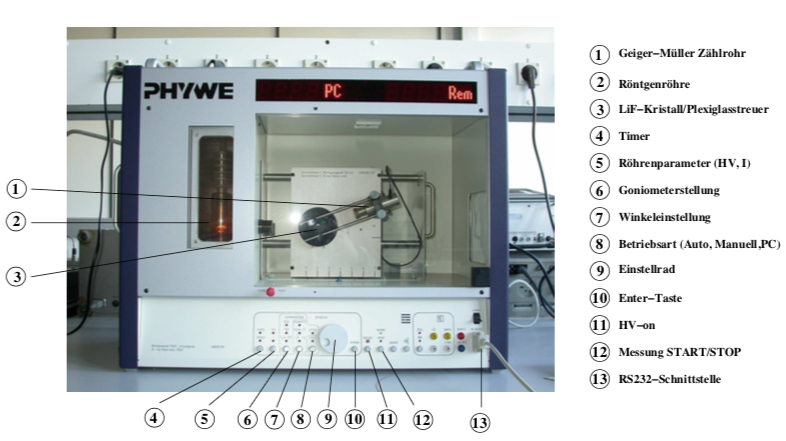
\includegraphics[width=\textwidth]{content/Versuchsaufbau.png}
  \caption{Versuchsaufbau \cite{1}.}
  \label{abb:2}
\end{figure}

Die Spektren werden mit einem Rechner aufgenommen. Für die Messungen muss immer eine
Beschleunigungsspannung von $U_b = \SI{35}{\kilo\volt}$ und ein Emissionsstrom von
$I = \SI{1}{\milli\ampere}$.

In dem ersten Teil des Versuchs soll die Bragg Bedingung überprüft werden. Dabei wird
ein fester Kristallwinkel von $\theta = 14^\circ$ eingestellt. Das Zählrohr soll sich
in einem Winkelbereich von $\alpha_{GM} = 26^\circ \text{bis} 30^\circ$ mit einem
Winkelzusatz von $\Delta \alpha = 0,1^\circ$ bewegen.

Bei der zweiten Messreihe wird das Emissionsspektrum der Kupferanode gemessen.
Dazu wird der Kristallwinkel und der Zählrohrwinkel gekoppelt. Der Winkelbereich
soll dabei $\theta = 4^\circ \text{bis} 26^\circ$ und in $0,2^\circ$ Schritten
gemessen werden. Dabei ist die Integrationszeit $\Delta t = 5 sec$.

Als letztes wird das Absorptionsspektrum von verschiedenen Materialien gemessen.
Dabei wird das zu messende Material vor das Geiger-Müller-Zählrohr gesetzt. Der Messbereich
muss für das jeweilige Material angepasst werden und in $0,1^\circ$ Schritten abgefahren werden.
Dabei ist die Integrationszeit $\Delta t = 20s$.
Die verwendeten Materialien sind Brom, Bismut, Strontium und Zirconium.
